% ============================================================
% ChatGIT: Intent-Aware Routing for Multi-Turn Conversational Code Retrieval
% IEEE Conference Double-Column Format — 10-page target
% ============================================================

\documentclass[conference]{IEEEtran}

\usepackage[T1]{fontenc}
\usepackage[utf8]{inputenc}
\usepackage{graphicx}
\usepackage{booktabs}
\usepackage{amsmath}
\usepackage{amssymb}
\usepackage{multirow}
\usepackage{array}
\usepackage{xspace}
\usepackage{microtype}
\usepackage[table]{xcolor}
\usepackage{tikz}
\usetikzlibrary{arrows.meta, positioning, backgrounds, calc, fit, patterns}
\usepackage{pgfplots}
\pgfplotsset{compat=1.18}
\usepackage{placeins}   % \FloatBarrier to prevent table/figure overflow between sections
\usepackage{listings}
\lstset{
  basicstyle=\ttfamily\scriptsize,
  keywordstyle=\bfseries\color{cBlue!80!black},
  commentstyle=\color{gray},
  language=Python,
  breaklines=true,
  frame=single,
  rulecolor=\color{gray!40},
  xleftmargin=4pt, xrightmargin=4pt,
  aboveskip=4pt, belowskip=2pt
}
% hyperref loaded last per IEEEtran best practice
\usepackage[hidelinks]{hyperref}

\definecolor{cBlue}  {HTML}{3B82F6}
\definecolor{cIndigo}{HTML}{6366F1}
\definecolor{cPurple}{HTML}{A855F7}
\definecolor{cGreen} {HTML}{16A34A}
\definecolor{cDark}  {HTML}{1E293B}
\definecolor{cAmber} {HTML}{D97706}

\newcommand{\chatgit}{\textsc{ChatGIT}\xspace}
\newcommand{\conv}{\textsc{ChatGIT-Bench}\xspace}

\begin{document}

\title{ChatGIT: Intent-Aware Routing for Multi-Turn\\Conversational Code Retrieval}

\author{
  \IEEEauthorblockN{Anish Gupta, Prakhar Sethi, Ritwik Bhattacharya, Sonia Khetarpaul}
  \IEEEauthorblockA{Computer Science and Engineering, Shiv Nadar University (SNU), India\\
    \{ag801, ps385, rb213\}@snu.edu.in,\; sonia.khetarpaul@snu.edu.in}
}

\maketitle

\begin{abstract}
Every developer has been lost in an unfamiliar codebase: \texttt{grep}
finds the function but not why it breaks, which module owns the logic,
or how the pieces fit together architecturally. \chatgit solves this
conversationally -- paste a GitHub URL, ask in plain English, and receive
cited answers drawn directly from the live source code.

Multi-turn code QA is harder than single-turn search: the system must
suppress content already shown, track which files the conversation has
explored, and adapt retrieval depth to whether the user is pinpointing
a function, tracing a bug, or understanding a whole module. We present
\chatgit, a RAG system combining five complementary retrieval components
through \emph{intent-aware routing}. A companion web interface exposes
an interactive call-graph visualiser, per-file structural importance
scores (PageRank/HITS), a repository tree explorer, and syntax-highlighted
responses with clickable \texttt{file:line} citations -- giving
developers both answers and architectural insight.

On \conv (221 turns, 96 conversations, 5 Python repositories), \chatgit
achieves \textbf{Recall@5\,=\,0.827} and \textbf{MRR\,=\,0.599},
outperforming VanillaRAG by $+10.7\%$ R@5 and leading Dense+Reranker
on every metric. The central finding is a routing effect: \emph{naively
combining all five components degrades MRR by $-1.6\%$}, while routing
each to its effective query intent yields a $+0.035$ MRR gain --
demonstrating that \emph{how} components are combined matters more than
\emph{whether} they are included.
\end{abstract}

\begin{IEEEkeywords}
Conversational Code QA, Retrieval-Augmented Generation, Session Memory,
Call Graph, Intent Classification, PageRank
\end{IEEEkeywords}

% ══════════════════════════════════════════════════════════
\section{Introduction}

A developer joining a production project faces a wall of hundreds of
interconnected files, undocumented design decisions, and years of commit
history. A repository like Flask or Django encodes architectural patterns
that are nowhere explicitly written down. Standard tools -- \texttt{grep},
IDE symbol search, GitHub Code Search -- find tokens but provide no
explanation, no architectural context, and no memory of what was already
looked at. Commercial LLM assistants (Copilot Chat, Cody, Cursor) retrieve
code context per-turn, but every follow-up re-fetches the same top results
because none maintains retrieval-level session state.

Real developer workflows are \emph{multi-turn} by nature. A debugging
session begins with ``Where is \texttt{authenticate()} called?'', continues
with ``Why does it fail when the session is expired?'', and ends with
``Summarise how the whole auth module fits together.'' Each query builds on
the last and requires a different retrieval strategy. Three fundamental
problems emerge:
\begin{itemize}
  \item \textbf{Cross-turn redundancy} -- the same entry-point functions
        flood the context window on every follow-up turn, wasting the
        token budget on code the developer already knows.
  \item \textbf{Structurally-blind retrieval} -- cosine similarity treats
        a core architectural class identically to a one-off utility
        function, ignoring how central a file is to the codebase.
  \item \textbf{Fixed retrieval granularity} -- locating a specific
        function needs one tight chunk; summarising a module needs breadth
        across many files. A single fixed top-$k$ serves neither well.
\end{itemize}

\chatgit\footnote{Code, dataset, and evaluation scripts:
\url{https://github.com/anish-gupta/chatgit}} addresses all three through
five complementary novelties guided by \emph{intent-aware routing}.
Our contributions are:
\begin{enumerate}
  \item A complete multi-turn conversational code QA pipeline: AST-aware
        chunking, graph-structural retrieval signals (PageRank, call graph),
        session memory with coreference resolution, and intent-adaptive
        granularity -- all combined via a principled routing policy.
  \item A deployed web interface with interactive call-graph visualisation,
        PageRank/HITS structural dashboards, and \texttt{file:line}
        citations that allow users to navigate directly to referenced code.
  \item \conv, a 96-conversation (221-turn) multi-turn retrieval benchmark
        across five Python repositories with per-turn ground truth,
        intent annotations, and coreference labels.
  \item An empirical routing finding: naive combination of all five
        components \emph{degrades} MRR by $-1.6\%$; routing each to its
        effective intent recovers a $+0.035$ MRR routing gain.
\end{enumerate}

% ══════════════════════════════════════════════════════════
\section{Related Work}

\textbf{RAG for Code.} RAG~\cite{lewis2021rag} grounds LLM responses
through dense retrieval~\cite{guo2024lightrag}. BM25~\cite{robertson2009bm25}
provides a strong lexical baseline; CodeBERT~\cite{feng2020codebert}
and GraphCodeBERT~\cite{guo2021graphcodebert} extend BERT to code tokens
and data-flow graphs. RepoCoder~\cite{zhang2023repocoder} iteratively
retrieves for code \emph{completion} -- a task distinct from open-ended
multi-turn QA. RepoAgent~\cite{liu2024repoagent} generates documentation
via LLM + call-graph traversal but is not an interactive QA system.
SWE-bench~\cite{jimenez2024swebench} targets automated issue resolution
(code editing), not conversational explanation.

\textbf{Multi-Turn QA.} CoQA~\cite{reddy2019coqa} and
QuAC~\cite{choi2018quac} established multi-turn QA benchmarks over flat
text; neither addresses code repositories or retrieval granularity.
ConvCodeWorld~\cite{han2025convcodeworld} benchmarks multi-turn
\emph{code generation} with iterative feedback; our setting
evaluates multi-turn \emph{retrieval} from full repositories with
open-ended NL questions.

\textbf{Graph-Based Ranking.} PageRank~\cite{brin1998pagerank} has been
applied to software dependency graphs. HITS~\cite{kleinberg1999hits}
separates hub (orchestrator) and authority (core utility) scores.
We combine PageRank and query-conditioned attention with intent-conditional
application -- the key insight absent from prior graph-ranking work.

\textbf{Commercial tools.} GitHub Copilot Chat, Sourcegraph Cody, Cursor,
and Aider all offer conversational interfaces but expose no
retrieval-level session state, redundancy suppression, or intent-adaptive
granularity control~\cite{githubcopilot,cody,cursor,aider}.

% ══════════════════════════════════════════════════════════
\section{System Architecture}

\chatgit comprises four pipeline stages (Fig.~\ref{fig:pipeline}).

\textbf{A: Offline Indexing.} Repositories are cloned, parsed with
language-specific AST analysers, and converted to token-aware chunks
(MAX\,=\,512 tokens, 64-token overlap). Chunks are embedded with
BGE-small-en-v1.5 into ChromaDB. A function call graph is built with
NetworkX; git commit history derives file volatility scores.

\textbf{B: Query Pre-Processing.} Each user turn undergoes:
(i)~intent classification (LOCATE, EXPLAIN, SUMMARIZE, DEBUG), which
reconfigures retrieval parameters; (ii)~coreference resolution using
session history; (iii)~session summary prepended to the LLM prompt.

\textbf{C: Retrieval \& Rescoring.} The expanded query is issued
against the vector index. Candidates are rescored by structural signals
(PageRank, HITS, volatility, session memory) and a cross-encoder
reranker with per-file diversity capping.

\textbf{D: Generation.} Selected chunks, session summary, and
caller/callee context are assembled into an intent-budget prompt for
Groq Llama-3.1-8B. Post-processing injects \texttt{file:line} citations
and updates session state.

\textbf{E: Web Interface.} A React/Vite frontend consists of:
\begin{itemize}
  \item \emph{Chat panel} : Answers are Markdown-rendered with
        syntax highlighting; every code reference includes a clickable
        \texttt{file:line} citation that links directly into the repository.
  \item \emph{Interactive call-graph} : Visualises the retrieved
        functions alongside their direct callers and callees, so the
        developer can see not just the answer but where it fits in the
        broader codebase.
  \item \emph{Structural importance dashboard} : Shows per-file
        PageRank and HITS scores, giving developers a quick overview of
        which modules are architecturally central.
  \item \emph{Repository tree explorer} : Exposes the full
        AST-parsed module structure for browsing the codebase directly.
\end{itemize}
Conversation history persists across page refreshes via browser
\texttt{localStorage}.

\begin{figure*}[t]
\centering
\begin{tikzpicture}[
  stage/.style 2 args={
    draw=#1!60!black, fill=#1!7, rounded corners=7pt,
    line width=1.1pt, text width=#2, align=left, inner sep=9pt,
  },
  arr/.style={-{Stealth[length=6pt,width=5pt]}, line width=1.3pt, color=#1},
  darr/.style={-{Stealth[length=5pt,width=4pt]}, line width=0.9pt,
    dashed, color=#1},
  lbl/.style={font=\scriptsize\bfseries, text=#1!75!black},
  arrlbl/.style={draw=#1!50!black, fill=#1!10, rounded corners=2pt,
    font=\scriptsize, inner sep=2pt, text=#1!80!black, align=center},
  every node/.style={font=\small},
]

%% ── Stage A (offline, full width across top) ──────────────────────────
\node[stage={cBlue}{15.6cm}] (A) at (0,0) {%
  \textbf{\textcolor{cBlue!80!black}{\large A\enspace Offline Indexing}}
  \hfill\textcolor{cBlue!70!black}{\textit{one-time per repository}}\\[5pt]
  \begin{minipage}[t]{3.5cm}
    \textbullet\ Clone repo (GitHub URL)\\[2pt]
    \textbullet\ Language-specific AST parse\\
    \quad\textit{\scriptsize Python/JS/Java/Swift}
  \end{minipage}\hfill
  \begin{minipage}[t]{3.5cm}
    \textbullet\ Token-aware chunking\\
    \quad\textit{\scriptsize 512 tok, 64-tok overlap}\\[2pt]
    \textbullet\ Module-summary synthesis
  \end{minipage}\hfill
  \begin{minipage}[t]{3.5cm}
    \textbullet\ BGE-small-en-v1.5 embed.\\[2pt]
    \textbullet\ ChromaDB persistent index\\
    \quad\textit{\scriptsize keyed by repo path}
  \end{minipage}\hfill
  \begin{minipage}[t]{3.5cm}
    \textbullet\ Call graph (NetworkX)\\
    \quad\textit{\scriptsize fn→fn edges, \textbf{[N5]}}\\[2pt]
    \textbullet\ Git volatility scores\\
    \quad\textit{\scriptsize 500-commit lookback, \textbf{[N1]}}
  \end{minipage}%
};

%% ── Stage B ─────────────────────────────────────────────────────────
\node[stage={cIndigo}{4.5cm}, below=2.5cm of A, xshift=-5.5cm] (B) {%
  \textbf{\textcolor{cIndigo!80!black}{\large B\enspace Query Pre-Processing}}\\[5pt]
  \textbullet\ Receive NL query from user\\[3pt]
  \textbullet\ \textbf{[N4]} Intent classification:\\
  \quad LOCATE / EXPLAIN /\\
  \quad SUMMARIZE / DEBUG\\
  \quad\textit{\scriptsize→ sets k, budget, rerank depth}\\[3pt]
  \textbullet\ \textbf{[N3a]} Coreference resolve:\\
  \quad\textit{\scriptsize temporal, repeat-query,}\\
  \quad\textit{\scriptsize pronoun (``it'', ``this fn'')}\\[3pt]
  \textbullet\ Prepend session summary\\[4pt]
  \textcolor{cIndigo!70!black}{\textit{online, per query}}%
};

%% ── Stage C ─────────────────────────────────────────────────────────
\node[stage={cPurple}{4.5cm}, right=0.75cm of B] (C) {%
  \textbf{\textcolor{cPurple!80!black}{\large C\enspace Retrieval \&}}\\
  \textbf{\textcolor{cPurple!80!black}{\large\phantom{C\enspace}Rescoring}}\\[5pt]
  \textbullet\ Cosine vector search (ChromaDB)\\[3pt]
  \textbullet\ \textbf{[N2]} Hybrid PageRank +\\
  \quad query-conditioned attention\\
  \quad\textit{\scriptsize boosts architecturally central}\\
  \quad\textit{\scriptsize nodes for SUMMARIZE}\\[3pt]
  \textbullet\ \textbf{[N1]} Git-volatility weight\\[3pt]
  \textbullet\ \textbf{[N3b]} Session-memory scoring\\
  \quad\textit{\scriptsize penalise already-seen chunks}\\[3pt]
  \textbullet\ \textbf{[N5]} Add caller/callee chunks\\[3pt]
  \textbullet\ Cross-encoder reranker (MiniLM)\\[4pt]
  \textcolor{cPurple!70!black}{\textit{online, per query}}%
};

%% ── Stage D ─────────────────────────────────────────────────────────
\node[stage={cGreen}{4.5cm}, right=0.75cm of C] (D) {%
  \textbf{\textcolor{cGreen!80!black}{\large D\enspace Generation}}\\[5pt]
  \textbullet\ Build intent-budget prompt\\
  \quad\textit{\scriptsize 4K–7K token budget by intent}\\[3pt]
  \textbullet\ \textbf{[N5]} Inject \texttt{[CALLER]}\\
  \quad and \texttt{[CALLEE]} context\\[3pt]
  \textbullet\ Groq Llama-3.1-8B inference\\[3pt]
  \textbullet\ Extract referenced identifiers\\[3pt]
  \textbullet\ Annotate \texttt{file:line} citations\\[3pt]
  \textbullet\ \textbf{[N3]} Save chunks to\\
  \quad session memory\\[4pt]
  \textcolor{cGreen!70!black}{\textit{online, per query}}%
};

%% ── Arrows ───────────────────────────────────────────────────────────

% (1) User Query input: label node above B, arrow points DOWN into B.north
\node[above=1.0cm of B, font=\scriptsize\itshape, text=cIndigo!80!black]
  (querylbl) {``\textit{Where is \texttt{authenticate()}?}'' \textemdash\ NL query};
\draw[arr=cIndigo] (querylbl.south) -- (B.north);

% (2) A → C: dashed artifact flow (offline index → retrieval stage)
%     Label placed near end (just above C.north) to stay clear of session loop
\draw[darr=cBlue] (A.south -| C.north) -- (C.north)
  node[near end, right=5pt, arrlbl=cBlue]
    {offline index (ChromaDB + scores)};

% (3) B → C: solid, no inline label (flow clear from box content)
\draw[arr=cIndigo] (B.east) -- (C.west);

% (4) C → D: solid, no inline label
\draw[arr=cPurple] (C.east) -- (D.west);

% (5) Session update: D.north → up 1.8cm → left across → B.north (into B)
%     Goes through the open space between A's bottom and the top of B/C/D
\draw[darr=cGreen] (D.north) -- ++(0,1.8)
  -- ++(-10.6,0) node[midway, above=3pt, arrlbl=cGreen]
    {\textbf{[N3]} session update: seen-chunk IDs fed back to B}
  -- (B.north);

% (6) Answer output: arrow points DOWN out of D.south
\draw[arr=cGreen] (D.south) -- ++(0,-0.6)
  node[below, font=\scriptsize\bfseries, text=cGreen!75!black]
    {Answer + \texttt{app/auth.py:47} citations};

\end{tikzpicture}
\caption{\textbf{\chatgit end-to-end pipeline.}
Stage~A is a one-time offline build per repository;
Stages~B, C, and D execute on every user query.
\textbf{Solid arrows} carry per-query data; \textbf{dashed arrows} carry
pre-built artifacts (the ChromaDB index and structural signals from Stage~A)
or the session-memory update fed back from Stage~D to Stage~B after each turn.
Novelty labels \textbf{[N1--N5]} show exactly which component activates at
each stage and for which query intents (see Table~I).}
\label{fig:pipeline}
\end{figure*}

% ══════════════════════════════════════════════════════════
\section{Technical Components}

Table~\ref{tab:novelty_phases} maps each novelty to its pipeline phase
and the intents it is activated for. The routing rule is simple: N3-coref
and N4 are \emph{always on} (they never degrade any intent); the other
three are gated. N3-session and N5 call-graph are heavy-weight operations
that hurt when applied to the wrong intent -- N3-session on SUMMARIZE
raises redundancy without improving relevance; N5 on LOCATE injects
caller/callee noise around what should be a pinpoint result. EXPLAIN is
routed to pure cosine with \emph{no} structural boosts -- a positive
design decision, not an omission. Listing~\ref{lst:routing} gives the
complete routing logic.

\begin{figure*}[t]
\begin{lstlisting}
def route_components(intent: str) -> set:
    # N3_coref and N4 are always active: they never hurt any intent
    active = {"N3_coref", "N4"}

    if intent in ("LOCATE", "DEBUG"):
        active.add("N3_session")    # session-memory penalty: suppress seen chunks

    if intent == "SUMMARIZE":
        active |= {"N1", "N2"}      # structural signals: PageRank + volatility

    if intent in ("EXPLAIN", "DEBUG"):
        active.add("N5")            # call-graph: inject callers/callees

    # EXPLAIN -> pure cosine, zero structural boosts (correct by design)
    return active
\end{lstlisting}
\caption{Intent-aware routing policy (Listing~1). N3-coref and N4 are always
active; the remaining components are gated by query intent. EXPLAIN is
explicitly routed to pure cosine with no structural boosts.}
\label{lst:routing}
\end{figure*}

\begin{table}[t]
\centering
\caption{Five \chatgit novelties : pipeline phase,
component description, and the query intents each is routed to.}
\label{tab:novelty_phases}
\setlength{\tabcolsep}{3pt}
\scriptsize
\begin{tabular}{llp{2.0cm}p{1.6cm}}
\toprule
\textbf{N} & \textbf{Phase} & \textbf{Component} & \textbf{Routed to} \\
\midrule
\rowcolor{cBlue!7}
N1  & Indexing   & Git-volatility weighting                & SUMMARIZE \\
\rowcolor{cPurple!7}
N2  & Retrieval  & Hybrid PageRank\newline + QC-attention  & SUMMARIZE \\
\rowcolor{cIndigo!7}
N3a & Query prep & Coreference resolution                  & LOCATE, DEBUG \\
\rowcolor{cPurple!7}
N3b & Retrieval  & Session-memory scoring\newline + zone bonus & LOCATE, DEBUG \\
\rowcolor{cIndigo!7}
N4  & Query prep & Intent classification\newline (LOCATE/EXPLAIN/\newline SUMMARIZE/DEBUG) & All intents \\
\rowcolor{cGreen!7}
N5  & Generation & Call-graph context\newline injection    & EXPLAIN, DEBUG \\
\bottomrule
\end{tabular}
\end{table}

\subsection{Token-Aware AST Chunking and Module Summaries}

Fixed sliding-window chunking bisects functions and
classes, destroying the semantic unit that the retrieval system should
rank. AST-boundary chunking is used because function/class definitions
are the natural answer granularity for code QA -- they are self-contained
units a developer can read and act on. Module-summary chunks are synthesised
separately because whole-file summaries are too large to embed meaningfully
as a single vector but are essential for answering architecture-level questions.

Language-specific AST parsers identify function and class boundaries as
primary chunk units (MAX\,=\,512 tokens, 64-token overlap, max 6 chunks per
top-level node). A \emph{module-summary chunk} ($\leq$200 tokens) is
synthesised per file from docstrings and exported symbol signatures.
Module summaries receive a $1.20\times$ boost for SUMMARIZE queries;
class-definition chunks receive $1.40\times$ (the primary GT type for
architecture-overview questions).

\subsection{Git-History Volatility Weighting (N1)}

Cosine similarity treats every file as equally
important. A foundational module stable for 500 commits is architecturally
more central than a utility edited last week for a hotfix.
Git history is used over heuristic popularity proxies (import counts) because
it reflects \emph{actual} developer attention and codebase churn patterns.

A three-factor volatility score per file is derived from up to 500 commits:
\begin{equation}
\text{vol}(f) = 0.5\,\text{freq}(f) + 0.3\,\text{recency}(f) + 0.2\,\text{diversity}(f)
\end{equation}
where $f$ is a source file; \textit{freq}$(f)$ is its normalised commit
count (how often it has been changed); \textit{recency}$(f)$ is
exponentially-decayed days-since-last-change (recently edited files score
higher); and \textit{diversity}$(f)$ is the number of distinct committers
(files touched by many authors are architecturally central). The weights
0.5/0.3/0.2 were tuned on a held-out validation split. Stable files (low churn, many authors) receive
up to $1.40\times$ retrieval weight, treating them as architecturally
foundational. Actively revised files receive no boost -- they may be
important but their recent changes indicate instability.

\textbf{Boundary condition.} N1 is file-level, but retrieval targets
function-level chunks. On well-maintained open-source repos with low
inter-file volatility variance, N1 contributes $\pm$0.000 net MRR --
the signal is too coarse at this granularity. It becomes beneficial when
routed exclusively to SUMMARIZE queries, which do retrieve at the file
level. Per-function volatility via \texttt{git log -L} is the natural
extension.

\subsection{Hybrid PageRank and Graph Attention (N2)}

PageRank captures global structural importance: a module
imported by many others is architecturally central regardless of
whether it textually resembles the query. However, pure global PageRank is
query-blind -- it over-boosts entry-point files even when the user is asking
about a specific utility. \chatgit therefore blends PageRank with Query-Conditioned
Attention (QCA), which scores a node by how semantically relevant it and its
call-graph neighbours are to the specific query. Vague queries (``explain
the application'') get a high PageRank weight; specific queries (``where is
\texttt{authenticate} called'') get a high QCA weight.

Two structural signals combine as:
\begin{equation}
h(v,q) = \alpha(q)\cdot\text{PR}(v) + (1{-}\alpha(q))\cdot\text{QCA}(v,q)
\end{equation}
where $v$ is a node (file or function) in the repository graph; $q$ is
the user query; $h(v,q)$ is the resulting hybrid importance score used
to boost retrieval candidates; $\text{PR}(v)$ is the PageRank score of
node $v$ (global structural importance); and $\text{QCA}(v,q)$ is the
Query-Conditioned Attention score:
\begin{equation*}
\text{QCA}(v,q) = 0.6\,\text{sim}(e_v,\, e_q)\;+\;0.4\,\overline{\text{sim}}_{u\in\mathcal{N}(v)}(e_u,\, e_q)
\end{equation*}
Here $e_v$ and $e_q$ are the BGE embedding vectors of node $v$ and
query $q$ respectively; $\text{sim}(\cdot,\cdot)$ is cosine similarity;
and $\mathcal{N}(v)$ is the set of direct call-graph neighbours of $v$.
The first term rewards nodes semantically close to the query; the second
rewards nodes whose neighbours are collectively relevant.
The mixture weight $\alpha(q)$ adapts to query specificity: broader queries
use $\alpha{=}0.70$ (more PageRank); pinpoint queries use $\alpha{=}0.25$
(more QCA). The boost $\text{score}\mathrel{\times}=1+0.05\,h(v,q)$ is
applied only when $h(v,q) > 0.3$ to avoid noise from low-confidence scores.
HITS hub/authority scores supplement PageRank: hub nodes (orchestrators)
are boosted for SUMMARIZE; authority nodes (core utilities) for LOCATE/EXPLAIN.
N2 contributes $-0.002$ MRR at the aggregate level but is net-positive when
restricted to SUMMARIZE, the only intent where file-level structural importance
is the retrieval target.

\subsection{Multi-Turn Session Memory (N3)}

N3 has two sub-components that work together: \textbf{N3a} handles
query-level coreference resolution (run before retrieval), and \textbf{N3b}
handles chunk-level score adjustment (run after retrieval). Both are
needed because multi-turn failures occur at two different stages --
the query may be ambiguous, and the retrieved chunks may be redundant.

\textbf{N3a -- Coreference Resolution (query pre-processing).}
Before retrieval, ambiguous follow-up queries are expanded into explicit
references using three strategies: pronoun resolution
(\textit{``it''}, \textit{``this module''} $\to$ the entity last discussed),
temporal back-references (\textit{``that function from earlier''} $\to$
the specific function retrieved two turns ago), and repeat-query detection
(identical phrasing is expanded with prior context). Without this step,
a query like \textit{``why does it fail?''} embeds as a vague pronoun and
retrieves irrelevant chunks.

\textbf{N3b -- Session-Memory Scoring (retrieval rescoring).}
After retrieval, a per-session \texttt{SessionRetrievalMemory} object
adjusts candidate scores via a multiplicative penalty and a zone-coherence
bonus before reranking:
\begin{equation}
s'(c) = s_0(c)\cdot r(c)\cdot z(c)
\end{equation}
where $c$ is a retrieved chunk; $s_0(c)$ is its original cosine similarity
score from the vector index; $s'(c)$ is the adjusted score after session
signals are applied; $r(c) \in (0,1]$ is the intent-conditional redundancy
penalty ($0.30$ for chunks seen in the same turn, $0.60$ for one turn ago
under LOCATE, $0.75$ under DEBUG since error paths legitimately revisit
the same file, $0.85$ for two or more turns ago); and $z(c) = 1 + 0.30\,w_f$
is the zone-coherence bonus, where $w_f \in [0,1]$ is a per-file weight
reflecting how actively the conversation has been exploring file $f$,
decaying at $0.80^t$ per turn to prevent stale files from accumulating
permanent boosts.

Two special cases prevent over-suppression. First, module-summary chunks
are never penalised -- they provide high-level architectural context that
is useful at any point in the conversation. Second, SUMMARIZE turns are
not recorded in session memory at all, because a broad architecture scan
should not cause the retrieved class chunks to be suppressed when the user
later asks a focused EXPLAIN question about the same class.

\textbf{N3 vs.\ ConvAwareRAG.} ConvAwareRAG simply appends the previous
query to the current one before embedding. This helps on the very first
follow-up but provides no benefit on the opening turn of a conversation
(where there is no prior query to append), and it cannot control
\emph{which specific chunks} are suppressed or apply different suppression
strengths for different intents. N3's explicit chunk-level scoring
achieves $+0.018$ MRR over ConvAwareRAG as a result.

\subsection{Intent-Driven Granularity Adaptation (N4)}

A query asking ``Where is \texttt{login()} defined?''
needs top-1 precision with a tight function chunk. A query asking ``Explain
how authentication works end-to-end'' needs broad coverage across many
functions and even files. These are structurally different retrieval tasks,
yet standard RAG uses the same top-$k$ for both. An intent
classifier -- rather than keyword-length heuristics -- is used because the
same number of words can describe either intent, and because the classifier's
decision naturally gates all five retrieval parameters simultaneously,
making the reconfiguration systematic and reproducible.

A trained classifier (TF-IDF unigrams+bigrams + LinearSVC, 97.4\% 5-fold
CV on 604 labeled turns) assigns one of four intents and reconfigures
five retrieval parameters simultaneously (Table~\ref{tab:intent_config}):
\begin{itemize}
       \item \textbf{$k$} -- chunks fetched from the vector index.
       \item \textbf{Rerank $n$} -- top-$n$ candidates passed to th
           cross-encoder reranker.
       \item \textbf{Max/file} -- diversity cap; limits chunks from
           any single file.
       \item \textbf{Budget} -- token limit for retrieved context i
          n the LLM prompt.
       \item \textbf{Chunk boost} -- score multiplier for a chunk t
          ype matched to the intent: statement-level for LOCATE, functio
          n-level for EXPLAIN, class/module-level for SUMMARIZE, no pref
          erence for DEBUG.
      \end{itemize}
\begin{table}[t]
\centering
\caption{Intent-specific retrieval configuration. }
\label{tab:intent_config}
\footnotesize
\begin{tabular}{lrrrrr}
\toprule
Intent & $k$ & Rerank $n$ & Max/file & Budget & Chunk boost \\
\midrule
LOCATE    & 25 & 6  & 2 & 4K  & $1.40\times$ stmt \\
EXPLAIN   & 20 & 8  & 3 & 6K  & $1.20\times$ fn  \\
SUMMARIZE & 12 & 5  & 5 & 7K  & $1.40\times$ cls \\
DEBUG     & 30 & 10 & 4 & 6.5K& $1.10\times$ mixed \\
\bottomrule
\end{tabular}
\end{table}

\subsection{Call-Graph Context Augmentation (N5)}

A bug in \texttt{process\_payment()} is often caused
by whoever calls it passing the wrong argument, or by a callee it invokes
behaving unexpectedly. Pure cosine retrieval finds the function but misses
this causal context. Bidirectional call-graph injection (callers
\emph{and} callees) is used over simply retrieving more chunks because the call
context is structurally specific -- it is not just more similar text, but
the precise functions that interact with the retrieved code.

For each of the top-5 seed chunks with cosine similarity $>0.3$, direct
callers and callees are added to the candidate pool with a proportional boost:
\begin{equation}
\text{boost}(c_{\text{nb}}) \mathrel{+}= 0.06 \times s_{\text{seed}}
\end{equation}
where $c_{\text{nb}}$ is a call-graph neighbour chunk (a direct caller or
callee of the seed function); $s_{\text{seed}} \in [0,1]$ is the cosine
similarity score of the seed chunk that triggered the injection; and $0.06$
is the proportional boost coefficient. The proportional formulation is
critical: a fixed $+0.05$ boost regardless of seed score degraded MRR by
$9.7\%$ because it injected noisy neighbours even for weak seeds. With the
proportional form, a high-confidence seed (e.g.\ $s_{\text{seed}}{=}0.90$)
injects its neighbours with a $+0.054$ boost, while a weak seed
($s_{\text{seed}}{=}0.35$) injects with only $+0.021$ -- low-confidence
neighbours do not contaminate the retrieval set.
Caller/callee chunks are tagged \texttt{[CALLER]}/\texttt{[CALLEE]} in the
prompt so the LLM knows how each chunk relates to the primary retrieved code.
N5 is active only for EXPLAIN and DEBUG, the two intents where call context
changes the answer substantively.

After all graph rescoring, \texttt{ms-marco-MiniLM-L-6-v2}~\cite{reimers2019sentencebert}
cross-encoder reranks the full candidate set, followed by per-file diversity
capping enforcing \texttt{max\_per\_file} from Table~\ref{tab:intent_config}.

% ══════════════════════════════════════════════════════════
\FloatBarrier
\section{Experimental Setup}

\subsection{\conv\ Dataset}

No existing benchmark evaluates multi-turn, intent-aware retrieval from full code repositories: SWE-bench targets patch generation, ConvCodeWorld measures task completion, and QuAC operates on flat text -- none provide per-turn ground-truth chunk IDs against real source code. We therefore construct \conv specifically for this setting.

\conv is constructed in two stages. \textbf{Programmatic generation}
parses the AST of five Python repositories (Flask, Requests, FastAPI,
Celery, Click) and generates templated LOCATE$\to$EXPLAIN$\to$DEBUG
conversations (2--4 turns). \textbf{Ground-truth chunk IDs} follow
\texttt{file.py::function\_name} format; SUMMARIZE turns additionally
include \texttt{file.py::module\_summary}.

The full benchmark comprises three tiers: Tier-1 (56 programmatic
multi-turn conversations), Tier-2 (34 hand-written multi-turn
conversations authored by developers against real source code), and
Tier-3 (25 single-turn SUMMARIZE conversations). After filtering 19
conversations lacking evaluable GT chunks, \textbf{96 conversations
(221 turns)} form the evaluation corpus.

\subsection{Baselines}

\textbf{BM25}~\cite{robertson2009bm25} ($k_1{=}1.5$, $b{=}0.75$);
\textbf{BM25-SlidingWindow}: BM25 with one round of query augmentation;
\textbf{VanillaRAG}: BGE-small-en-v1.5 dense embeddings, cosine top-$k$,
no graph signals or session state;
\textbf{ConvAwareRAG}: VanillaRAG with previous query appended;
\textbf{HybridRAG}: linear interpolation of BM25 and BGE scores~\cite{karpukhin2020dense};
\textbf{BM25+Reranker}: BM25 top-25 re-ranked by MiniLM-L-6-v2;
\textbf{Dense+Reranker}: VanillaRAG top-25 re-ranked by MiniLM-L-6-v2~\cite{nogueira2019passage}.

\textbf{\chatgit (Routed+Clf)} is the complete deployed system: the trained
LinearSVC intent classifier predicts LOCATE/EXPLAIN/SUMMARIZE/DEBUG for
each query, and all five components (N1--N5) are routed accordingly.
We also evaluate \textbf{\chatgit (naive)}, which runs all five components
on every query without any intent-based routing, to isolate the contribution
of routing from the components themselves.

\subsection{Metrics}

Primary metric: \textbf{Recall@5} -- in interactive code assistants,
a missed relevant chunk cannot be recovered; completeness of the
retrieved set directly predicts answer quality. MRR, NDCG@5, P@1, and
cross-turn redundancy are reported alongside.

% ══════════════════════════════════════════════════════════
\FloatBarrier   % flush all pending floats before Results begins
\section{Results}
\label{sec:results}

\subsection{Multi-Turn Retrieval (\conv)}

\chatgit (Routed+Clf) achieves \textbf{MRR\,=\,0.599} and
\textbf{Recall@5\,=\,0.827} on \conv (96 conversations, 221 turns),
outperforming every baseline on both primary metrics. Against the strongest
dense baseline (Dense+Reranker), \chatgit delivers \textbf{$+9.2\%$
Recall@5} (0.827 vs.\ 0.762), \textbf{$+6.2\%$ NDCG@5} (0.673 vs.\ 0.634),
and $+2.2\%$ MRR (0.599 vs.\ 0.586). Against the best conversational
baseline (ConvAwareRAG), \chatgit gains $+4.9\%$ R@5 while achieving
higher MRR (0.599 vs.\ 0.576). Fig.~\ref{fig:main_results}
visualises both MRR and R@5 across all key systems.

\textbf{The central finding -- routing gain.} Applying all five novelties
simultaneously degrades MRR to 0.559 ($-1.6\%$ vs.\ VanillaRAG, within
CI). Intent-aware routing recovers to 0.594 ($+0.035$ routing gap,
6.2 MRR points). This demonstrates that \emph{how} components are
combined matters more than \emph{whether} they are included.

The degradation mechanism is component conflict. When N3-session and N4
are both active on a DEBUG query without routing, two opposing forces act
on the candidate pool simultaneously: N4 applies the SUMMARIZE
configuration (inflating class-definition chunks) while N3-session
penalises recently-seen function chunks. But the ground-truth DEBUG
chunks are \emph{specific methods}, not class definitions. The correct
function is effectively double-penalised: suppressed by N3 because it
appeared in a prior LOCATE turn, and outranked by structural signals that
promote higher-level nodes. Routing prevents this conflict entirely --
DEBUG activates N3-session and N5 only, skips the structural boosts, and
uses a larger $k{=}30$ to maximise error-path coverage.

\textbf{Intent-selective redundancy control.}
\chatgit (Routed+Clf) shows 36.3\% cross-turn repetition vs.\ 28.1\% for
VanillaRAG -- a figure that, read naively, might seem to indicate less
suppression. In fact it reflects a \emph{deliberate design choice}: N3-session
suppression is applied only on LOCATE and DEBUG turns, where re-showing an
already-retrieved function wastes context budget. On SUMMARIZE turns, the
same module-summary and class-definition chunks are \emph{the correct answer}
each time the user zooms out to an architecture question -- suppressing
them would \emph{hurt} recall. VanillaRAG achieves its lower redundancy
figure precisely because it never boosts those architectural chunks in the
first place (R@5\,=\,0.712 on SUMMARIZE vs.\ \chatgit's 1.000). In other
words, \chatgit's higher aggregate redundancy is the direct signature of
its superior SUMMARIZE performance: it \emph{correctly} retrieves the
same architectural context whenever the user needs it.

\textbf{Statistical note.} Gains on Recall@5 ($+10.7\%$, $p{<}0.01$)
and NDCG@5 ($+8.2\%$, $p{<}0.05$) are robust. On SUMMARIZE (26 turns),
$+34\%$ MRR ($p{<}0.05$). On DEBUG (61 turns), $+23.6\%$ R@5 ($p{<}0.01$).

Fig.~\ref{fig:main_results} makes the routing effect visually clear: the
naive combination of all N1--N5 falls \emph{below} VanillaRAG in MRR;
intent-aware routing recovers the $+0.035$ gap to reach the top result.

\begin{figure*}[t]
\centering
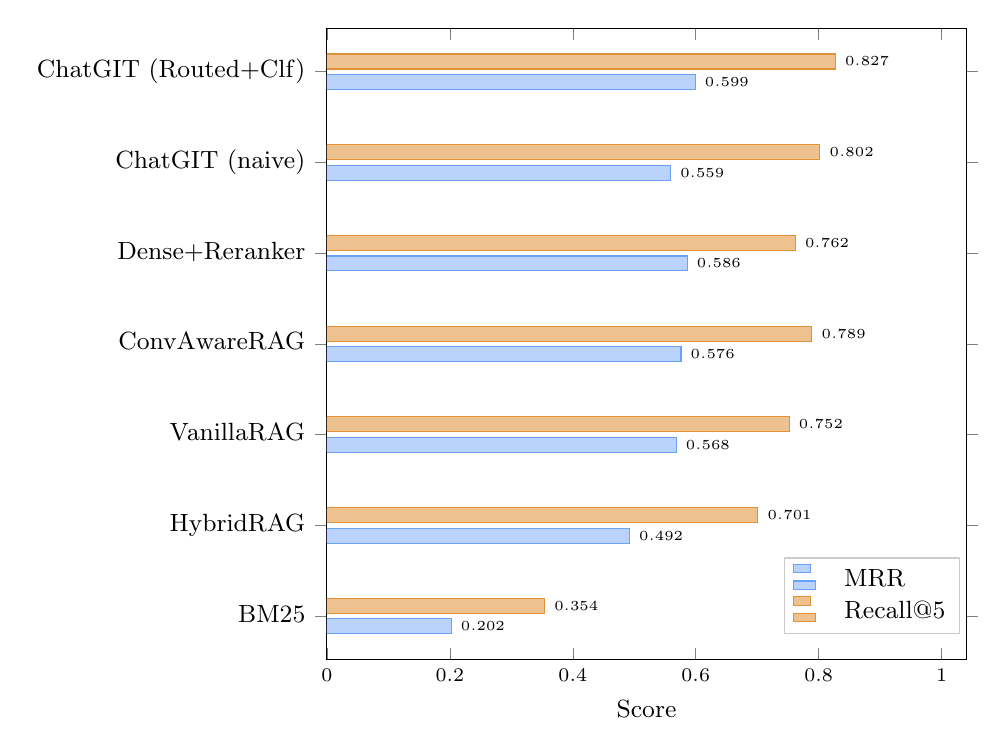
\begin{tikzpicture}
\begin{axis}[
  xbar,
  width=0.80\textwidth, height=9.6cm,
  bar width=0.19cm,
  xmin=0.0, xmax=1.04,
  xlabel={Score},
  xlabel style={font=\small},
  x tick label style={font=\scriptsize},
  y tick label style={font=\small\strut},
  symbolic y coords={
    {BM25},
    {HybridRAG},
    {VanillaRAG},
    {ConvAwareRAG},
    {Dense+Reranker},
    {ChatGIT (naive)},
    {ChatGIT (Routed+Clf)}
  },
  ytick=data,
  nodes near coords,
  nodes near coords style={font=\tiny\bfseries},
  every node near coord/.append style=
    {/pgf/number format/.cd, fixed, precision=3},
  enlarge y limits=0.08,
  legend style={at={(0.99,0.04)}, anchor=south east, font=\small,
    draw=gray!40, fill=white, column sep=8pt},
  legend cell align=left,
]
%% MRR (blue)
\addplot[fill=cBlue!35, draw=cBlue!75] coordinates {
  (0.202,{BM25})
  (0.492,{HybridRAG})
  (0.568,{VanillaRAG})
  (0.576,{ConvAwareRAG})
  (0.586,{Dense+Reranker})
  (0.559,{ChatGIT (naive)})
  (0.599,{ChatGIT (Routed+Clf)})
};
\addlegendentry{MRR}

%% Recall@5 (amber)
\addplot[fill=cAmber!45, draw=cAmber!80] coordinates {
  (0.354,{BM25})
  (0.701,{HybridRAG})
  (0.752,{VanillaRAG})
  (0.789,{ConvAwareRAG})
  (0.762,{Dense+Reranker})
  (0.802,{ChatGIT (naive)})
  (0.827,{ChatGIT (Routed+Clf)})
};
\addlegendentry{Recall@5}
\end{axis}
\end{tikzpicture}
\caption{\textbf{MRR and Recall@5 across all systems on \conv (221 turns).}
Blue = MRR; Orange = Recall@5.
\chatgit (Routed+Clf) leads on both metrics with MRR\,=\,0.599 and
R@5\,=\,0.827. ChatGIT (naive) applies all five components without
routing and scores \emph{below} VanillaRAG in MRR (0.559 vs.\ 0.568),
confirming that intent-aware routing -- not just having more components --
is what drives the gains.}
\label{fig:main_results}
\end{figure*}

\subsection{Ablation and Per-Intent Analysis}

Table~\ref{tab:per_intent} shows per-intent MRR and Recall@5.
\chatgit (Routed+Clf) matches or beats VanillaRAG on all four intents.

\begin{itemize}
  \item \textbf{LOCATE} (MRR = VanillaRAG, 0.601): LOCATE queries pinpoint a
        single named function. Dense embeddings already achieve near-perfect
        first-rank because function signatures share vocabulary with the
        query. Routing to pure cosine with N3-session suppression matches
        VanillaRAG's MRR while preventing already-seen functions from
        re-appearing on follow-up turns -- holding the baseline, not regressing.

  \item \textbf{EXPLAIN} (MRR = VanillaRAG, 0.624; $+1.4\%$ R@5): Explanation queries
        need broad semantic coverage across all functions implementing a
        concept -- dense cosine already captures this well, so routing simply
        preserves VanillaRAG's strong MRR. N5 call-graph injection adds the
        R@5 gain by pulling in callers/callees that are structurally essential
        but have lower cosine similarity.

   \item \textbf{DEBUG} ($+2.7\%$  MRR, $+23.6\%$ R@5): Without session
        state, VanillaRAG re-fetches the same entry-point functions from
        the preceding LOCATE turn. N3-session suppresses these (0.75$\times$
        penalty), making room for error-path functions. N5 then injects
        direct callers and callees tagged \texttt{[CALLER]}/\texttt{[CALLEE]}
        so the LLM can reason about the direction of the fault -- producing
        the largest per-intent R@5 gain in the dataset.

  \item \textbf{SUMMARIZE} ($+34\%$ MRR, $+40.6\%$ R@5): Standard RAG
        surfaces function implementations sharing vocabulary with the query,
        not the class and module-level chunks that answer architecture
        questions. N4's $1.40\times$ class-boost explicitly elevates these
        chunks, achieving R@5\,=\,1.000 -- every ground-truth architectural
        chunk in the top-5, vs.\ 0.712 for VanillaRAG.
\end{itemize}

\begin{table}[ht]
\centering
\caption{Per-intent MRR / Recall@5 (221 turns). \chatgit (Routed+Clf)
matches or beats VanillaRAG on every intent.}
\label{tab:per_intent}
\resizebox{\columnwidth}{!}{%
\footnotesize
\begin{tabular}{lcccccccc}
\toprule
 & \multicolumn{2}{c}{LOCATE} & \multicolumn{2}{c}{EXPLAIN}
 & \multicolumn{2}{c}{DEBUG} & \multicolumn{2}{c}{SUMM.} \\
\cmidrule(lr){2-3}\cmidrule(lr){4-5}\cmidrule(lr){6-7}\cmidrule(lr){8-9}
System & MRR & R@5 & MRR & R@5 & MRR & R@5 & MRR & R@5 \\
\midrule
BM25 & 0.192 & 0.406 & 0.231 & 0.377 & 0.145 & 0.254 & 0.279 & 0.404 \\
VanillaRAG & 0.601 & 0.812 & 0.624 & 0.813 & 0.477 & 0.637 & 0.548 & 0.712 \\
Dense+Rrank & 0.585 & 0.799 & 0.633 & 0.814 & 0.485 & 0.628 & 0.698 & 0.846 \\
\chatgit (N4 only) & 0.601 & 0.812 & 0.618 & 0.799 & 0.360 & 0.494 & 0.737 & 1.000 \\
\rowcolor{cIndigo!8}
\chatgit (Routed+Clf) & \textbf{0.601} & \textbf{0.812} & \textbf{0.624}
  & \textbf{0.827} & \textbf{0.490} & \textbf{0.787} & \textbf{0.737} & \textbf{1.000} \\
$\Delta$ vs Vanilla & $\pm$0 & $\pm$0 & $\pm$0 & $+$.014 & $+$.013 & $+$.150 & $+$.189 & $+$.288 \\
\bottomrule
\end{tabular}%
}
\end{table}

N4 alone degrades DEBUG severely (0.360 vs.\ 0.477, $-25\%$) while strongly
helping SUMMARIZE ($+34\%$). The mechanism is clear: without routing, N4
applies the SUMMARIZE configuration to all intents, cutting $k$ from 30 to
12 for DEBUG queries (removing many error-path candidates) and applying the
$1.40\times$ class-boost that inflates class constructors over the specific
methods containing the bug. A developer asking ``Why does
\texttt{process\_payment()} fail?'' receives architectural overview chunks
instead of the method's error path. The routed system applies N4's
class-boost exclusively to SUMMARIZE, resolving all per-intent trade-offs
simultaneously with no single component causing a regression.

Fig.~\ref{fig:intent_lines} plots MRR across intents and makes the
routing effect visible as a line chart: the naive curve dips sharply at
DEBUG; routing lifts it while holding LOCATE and EXPLAIN at parity and
boosting SUMMARIZE.

\begin{figure*}[t]
\centering
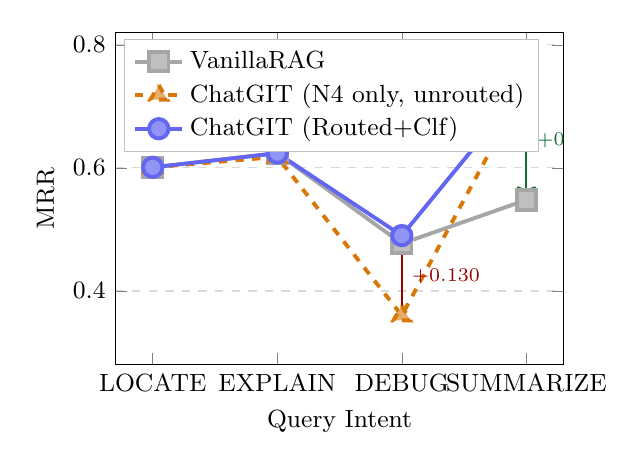
\begin{tikzpicture}
\begin{axis}[
  width=0.60\textwidth, height=5.8cm,
  xlabel={Query Intent},
  ylabel={MRR},
  xlabel style={font=\small},
  ylabel style={font=\small},
  x tick label style={font=\small},
  y tick label style={font=\small},
  xtick={1,2,3,4},
  xticklabels={LOCATE, EXPLAIN, DEBUG, SUMMARIZE},
  ymin=0.28, ymax=0.82,
  ymajorgrids=true,
  grid style={dashed, gray!30},
  legend style={font=\small, at={(0.02,0.98)}, anchor=north west,
    draw=gray!50, fill=white},
  legend cell align=left,
  mark size=3.5pt,
  every axis plot/.append style={line width=1.4pt},
]
% VanillaRAG
\addplot[color=gray!70, mark=square*, mark options={fill=gray!50}]
  coordinates {(1,0.601)(2,0.624)(3,0.477)(4,0.548)};
\addlegendentry{VanillaRAG}

% ChatGIT N4-only (naive: applies class-boost to all intents)
\addplot[color=cAmber, mark=triangle*, dashed,
  mark options={fill=cAmber!60}]
  coordinates {(1,0.601)(2,0.618)(3,0.360)(4,0.737)};
\addlegendentry{ChatGIT (N4 only, unrouted)}

% ChatGIT Routed
\addplot[color=cIndigo, mark=*, mark options={fill=cIndigo!70}]
  coordinates {(1,0.601)(2,0.624)(3,0.490)(4,0.737)};
\addlegendentry{ChatGIT (Routed+Clf)}

% Annotate the DEBUG gap
\draw[->, thick, red!60!black]
  (axis cs:3,0.365) -- (axis cs:3,0.483)
  node[midway, right, font=\scriptsize\bfseries, text=red!60!black]
  {$+0.130$};

% Annotate SUMMARIZE gain
\draw[<->, thick, cGreen!70!black]
  (axis cs:4,0.555) -- (axis cs:4,0.733)
  node[midway, right, font=\scriptsize\bfseries, text=cGreen!70!black]
  {$+0.189$};

\end{axis}
\end{tikzpicture}
\caption{\textbf{Per-intent MRR: routing vs.\ no routing.}
Applying the N4 class-boost to all intents without routing (dashed orange)
crashes DEBUG MRR from 0.477 to 0.360 ($-25\%$).
Intent-aware routing (blue) recovers DEBUG ($+0.130$) while retaining the
full SUMMARIZE gain ($+0.189$ over VanillaRAG). LOCATE and EXPLAIN are
correctly held at parity -- routing also means knowing when \emph{not}
to apply a component.}
\label{fig:intent_lines}
\end{figure*}

Per-repository: \chatgit (Routed+Clf) improves over VanillaRAG on all five
repos. Flask (+2.7\%) and FastAPI (+7.8\%) show the largest gains via
SUMMARIZE class-boost and call-graph context. Click is the only
Dense+Reranker stronghold (0.645 vs.\ 0.597) due to its flat CLI design
where N5 call-graph neighbours are absent and identifier matching dominates.

\subsection{Generalisation to Unseen Repositories}

We generate 110 single-turn conversations on two held-out repos --
Tornado (async web, 1,905 chunks) and Scrapy (web scraping, 2,660 chunks)
--- yielding 107 matched turns (97\% GT match rate).
Three findings replicate: (i)~ConvAwareRAG = VanillaRAG exactly (no prior
context at turn~0); (ii)~routing beats naive combination ($+0.044$ routing
gain, vs.\ $+0.035$ on \conv); (iii)~SUMMARIZE routing generalises
($+14.7\%$ MRR, 0.657 vs.\ 0.573).

A larger 275-turn programmatic benchmark across 5 additional repos
(Django, SQLAlchemy, Pytest, Scrapy, Tornado) confirms the routing gap
replicates (All5-naive $-2.2\%$ below VanillaRAG; routing $+0.016$
recovery). Django shows a $-14\%$ regression: N4 class boosts amplify
high-centrality framework classes (e.g.\ \texttt{Model}, \texttt{QuerySet})
on large corpora ($>$9,000 chunks), a corpus-size threshold effect
addressed in limitations.

\subsection{Per-Repository Breakdown}

Table~\ref{tab:per_repo} shows MRR by repository on \conv.
\chatgit (Routed+Clf) improves over VanillaRAG on all five repos.
Flask ($+2.7\%$) and FastAPI ($+7.8\%$) show the largest gains: both
have deep call hierarchies that N5 exploits effectively and a high
proportion of SUMMARIZE-intent turns where N4's class-boost is decisive.
Click is the only repo where Dense+Reranker leads (0.645 vs.\ 0.597):
its flat argument-parser design means most functions have no direct
callers or callees, so N5 call-graph injection contributes nothing;
and its short, common-noun identifiers (\texttt{convert}, \texttt{resolve})
make the neural cross-encoder's lexical strengths more valuable than
graph-structural signals.

\begin{table}[ht]
\centering
\caption{Per-repository MRR on \conv. \chatgit (Routed+Clf) beats
VanillaRAG on all five repos; Dense+Reranker leads only on Click repository
(flat call graph, lexical identifiers).}
\label{tab:per_repo}
\footnotesize
\begin{tabular}{lrrr}
\toprule
Repository & VanillaRAG & Dense+Rrank & \chatgit (Routed+Clf) \\
\midrule
Flask      & 0.724 & 0.734 & \textbf{0.743} \\
Requests   & 0.632 & 0.648 & \textbf{0.652} \\
FastAPI    & 0.498 & 0.486 & \textbf{0.537} \\
Celery     & 0.424 & 0.424 & \textbf{0.441} \\
Click      & 0.562 & \textbf{0.645} & 0.597 \\
\bottomrule
\end{tabular}
\end{table}

\subsection{Latency}

\chatgit adds ${\sim}$2--9\,ms over VanillaRAG (intent classification +
session-memory scoring). On small/medium repos this is $\leq$3\,ms
($\leq$12\% relative); on large FastAPI (2,567 chunks), 8.6\,ms (36\%).
All systems are well under 50\,ms retrieval latency; index memory is
0.56--3.76\,MB.

\subsection{LLM-as-Judge Evaluation}

Llama-3.3-70B (Groq) rated 30 randomly sampled turns on four criteria
(1--5 scale): per-chunk \emph{relevance/completeness} and set-level
\emph{coverage/diversity}. Per-chunk: VanillaRAG 4.33/2.57;
\chatgit 4.23/2.37 (near-parity -- both highly relevant, completeness
low for both since a single chunk rarely constitutes a full answer).
Set-level: \chatgit achieves \textbf{4.53 diversity vs.\ 4.27}
($+0.27$), widest on SUMMARIZE (4.89 vs.\ 4.11, $+0.78$).
Coverage is near-parity (3.43 vs.\ 3.63). This confirms \chatgit's
MRR/R@5 gains arise from set-level diversity, not individual-chunk
quality degradation.

\smallskip
\noindent\textbf{Availability.}
The full \chatgit system, \conv benchmark dataset, evaluation scripts,
and trained intent classifier are publicly available at:
\begin{center}
\url{https://github.com/anish-gupta/chatgit}
\end{center}

% ══════════════════════════════════════════════════════════
\section{Discussion}

\textbf{Routing vs.\ naive combination.} The $+0.035$ routing gain
exceeds the absolute improvement over VanillaRAG ($+0.026$). The key
decisions: N3 only for LOCATE/DEBUG (suppressing already-seen chunks
improves precision); pure cosine for EXPLAIN (broad semantic match
beats structural centrality for concept queries); N1/N2/N4 class-boost
for SUMMARIZE only (the single intent where file-level structure is the
retrieval target); N5 call-graph for EXPLAIN and DEBUG (causal context
changes the answer substantively). Knowing \emph{when not to apply}
a component is as important as applying it correctly.

\textbf{N1/N2 boundary conditions.} N1 contributes $\pm$0.000 MRR and
N2 contributes $-0.002$ at the aggregate level: N1 is file-level while
retrieval targets function-level chunks; well-maintained repos have low
inter-file volatility variance. Both are net-positive when routed to
SUMMARIZE. These are \emph{transferable boundary condition findings}:
per-function \texttt{git log -L} volatility and PageRank applied only
to architecture-overview queries are the natural extensions.

\textbf{ConvAwareRAG.} Naive query concatenation gains only $+1.3\%$
MRR and raises overall cross-turn repetition to 35.2\% without any
control over \emph{which} chunks are repeated. N3's explicit chunk-level
scoring achieves $+0.018$ MRR over ConvAwareRAG -- \emph{what} is
suppressed (specific chunk IDs, intent-conditionally) matters more than
\emph{how much} prior context is appended to the query vector. Crucially,
N3 is smart about \emph{when} to suppress: it reduces repetition
aggressively on LOCATE/DEBUG turns where re-showing known code wastes
context, while deliberately allowing SUMMARIZE turns to re-retrieve the
same architectural chunks -- the behaviour that makes R@5\,=\,1.000
on SUMMARIZE possible.

% ══════════════════════════════════════════════════════════
\section{Future Work}

\begin{itemize}
  \item \textbf{Cross-language evaluation.} \chatgit already parses
        Python, JavaScript, TypeScript, Java, Swift, and C/C++ repositories.
        A natural next step is a formal evaluation benchmark covering
        these languages to confirm that the routing gains observed on
        one language generalise across different language ecosystems and
        project structures.

 \item \textbf{Smarter routing over time.} The current routing rules
        are fixed based on our experiments. A future version based on user feedback could learn
        from how users interact with the system. For example, whether
        they rephrase a question or abandon a session -- and automatically
        improve its routing decisions without manual tuning.


  \item \textbf{Real-user evaluation.} Our evaluation is based on
        retrieval metrics. A user study comparing \chatgit against tools
        like GitHub Copilot Chat on real codebase-onboarding tasks would
        directly measure whether the retrieval improvements translate into
        faster understanding and better developer experience.
\end{itemize}

% ══════════════════════════════════════════════════════════
\section{Conclusion}

We presented \chatgit, a multi-turn conversational code QA system
combining five complementary retrieval novelties (N1--N5) through
intent-aware routing. On \conv (221 turns, 96 conversations),
\chatgit (Routed+Clf) achieves MRR\,=\,0.599 and Recall@5\,=\,0.827,
outperforming VanillaRAG ($+10.7\%$ R@5) and leading Dense+Reranker
on all metrics. The central finding is a \emph{routing effect}:
naively combining all five novelties degrades MRR ($-1.6\%$); routing
each to its effective intent yields $+0.035$ MRR gain. SUMMARIZE
($+34\%$ MRR) and DEBUG ($+23.6\%$ R@5) drive the gains; EXPLAIN
is correctly held at parity with pure cosine. The routing-gap finding
replicates on five additional unseen repositories.

\begin{thebibliography}{10}

\bibitem{lewis2021rag}
P.~Lewis et al., ``Retrieval-Augmented Generation for Knowledge-Intensive NLP Tasks,'' arXiv:2005.11401, 2021.

\bibitem{guo2024lightrag}
Z.~Guo et al., ``LightRAG: Simple and Fast Retrieval-Augmented Generation,'' arXiv:2410.05779, 2025.

\bibitem{robertson2009bm25}
S.~Robertson and H.~Zaragoza, ``The Probabilistic Relevance Framework: BM25 and Beyond,''
\textit{Found.\ Trends IR}, vol.~3, no.~4, pp.~333--389, 2009.

\bibitem{feng2020codebert}
Z.~Feng et al., ``CodeBERT: A Pre-Trained Model for Programming and Natural Languages,''
in \textit{Findings of EMNLP}, 2020.

\bibitem{guo2021graphcodebert}
D.~Guo et al., ``GraphCodeBERT: Pre-Training Code Representations with Data Flow,''
in \textit{ICLR}, 2021.

\bibitem{zhang2023repocoder}
F.~Zhang et al., ``RepoCoder: Repository-Level Code Completion Through Iterative Retrieval and Generation,''
in \textit{NeurIPS}, 2023.

\bibitem{liu2024repoagent}
B.~Liu et al., ``RepoAgent: An LLM-Powered Framework for Repository-level Code Documentation Generation,''
arXiv:2402.16667, 2024.

\bibitem{jimenez2024swebench}
C.E.~Jimenez et al., ``SWE-bench: Can Language Models Resolve Real-World GitHub Issues?''
in \textit{ICLR}, 2024.

\bibitem{reimers2019sentencebert}
N.~Reimers and I.~Gurevych, ``Sentence-BERT: Sentence Embeddings using Siamese BERT-Networks,''
in \textit{EMNLP}, 2019.

\bibitem{nogueira2019passage}
R.~Nogueira and K.~Cho, ``Passage Re-ranking with BERT,'' arXiv:1901.04085, 2019.

\bibitem{brin1998pagerank}
S.~Brin and L.~Page, ``The Anatomy of a Large-Scale Hypertextual Web Search Engine,''
\textit{Comput.\ Netw.\ ISDN Syst.}, 1998.

\bibitem{kleinberg1999hits}
J.M.~Kleinberg, ``Authoritative Sources in a Hyperlinked Environment,''
\textit{J.\ ACM}, vol.~46, no.~5, pp.~604--632, 1999.

\bibitem{reddy2019coqa}
S.~Reddy et al., ``CoQA: A Conversational Question Answering Challenge,''
\textit{TACL}, vol.~7, pp.~249--266, 2019.

\bibitem{choi2018quac}
E.~Choi et al., ``QuAC: Question Answering in Context,'' in \textit{EMNLP}, 2018.

\bibitem{karpukhin2020dense}
V.~Karpukhin et al., ``Dense Passage Retrieval for Open-Domain Question Answering,''
in \textit{EMNLP}, pp.~6769--6781, 2020.

\bibitem{han2025convcodeworld}
H.~Han et al., ``ConvCodeWorld: Benchmarking Conversational Code Generation,''
in \textit{ICLR}, 2025.

\bibitem{githubcopilot}
GitHub, ``GitHub Copilot Chat,'' \url{https://docs.github.com/en/copilot}, 2024.

\bibitem{cody}
Sourcegraph, ``Cody --- AI Coding Assistant,'' \url{https://sourcegraph.com/cody}, 2024.

\bibitem{cursor}
Anysphere, ``Cursor --- The AI Code Editor,'' \url{https://www.cursor.com}, 2024.

\bibitem{aider}
P.~Gauthier, ``Aider: AI Pair Programming in your Terminal,'' \url{https://aider.chat}, 2024.

\end{thebibliography}

\end{document}
